%!TEX root = ../main.tex

\chapter{Design and Implementation}
\label{chap:design_and_implementation}
This chapter describes the process of producing and tuning the main component of the artefact --- the URL classifier. The first section of the chapter presents the findings of GSB's evaluation, the result of which constitutes the minimum acceptable classification accuracy.

The following two sections briefly describe the list-based module and explore machine-learning module of the artefact. Next, an initial performance analysis is carried out, which sets the scene for further parameter optimisation. Finally, the components mentioned above are brought together and assessed as a whole.

\section{Threshold definition}
Before attempting to improve the level of protection offered by the most popular browsers, GSB's classification accuracy needs to be assessed. In doing so, user behaviour will be simulated using a browser automation framework for accessing the phishing websites. The outcome of this serves as an accuracy threshold for the proposed artefact.

The first step of the process is data acquisition. A list of URLs pointing to online phishing webpages, confirmed to be malicious by the PhishTank community is fetched from their archive. The first test runs on the data available on the 1st of April. Testing a total number of 9345 phishing URLs, GSB managed to achieve a total accuracy of 50.76\%.
The next test is run with the data published on the 5th of April. This time GSB performed slightly worse, reporting 48.32\% accuracy on the 8164 phishing URLs. Running the same test on the data acquired on the 1st of April shows a significant drop in accuracy, reporting 40.28\% accuracy on 9359 URLs.
One notable mention is that because Google Chrome is resource demanding software, the results are altered by the fact that the testing phase of a dataset takes around eight hours. During this time, it has opportunities to update its URL hashes database.

Shifting the testing method to Google Safe Browsing API, the protection rate is slightly lower (Table \ref{tab:GSBAPI_RESULTS}). Finally, the threshold is set to be the average of all test results of 45.74\%.


\begin{singlespace}
	\begin{center}
		\begin{tabular}{ m{10em} m{10em} } \toprule
			\textbf{Date}        & \textbf{True-positive rate} \\ \midrule

			\textbf{05 May 2020} & 44.34\%                     \\

			\textbf{06 May 2020} & 44.33\%                     \\

			\textbf{07 May 2020} & 44.94\%                     \\

			\textbf{08 May 2020} & 45.34\%                     \\

			\textbf{09 May 2020} & 45.33\%                     \\

			\textbf{10 May 2020} & 43.60\%                     \\ \bottomrule
		\end{tabular}
		\captionsetup{type=table}\caption{Google Safe Browsing API test results}
		\label{tab:GSBAPI_RESULTS}
	\end{center}
\end{singlespace}


\section{List-based module}
It is safe to assume that most of web browsing activity takes place across a limited set of domains. This is reflected in the existence of domain rankings of most popular domains. Because these are known to be benign, there is no reasoning for wasting resources on the classification process. A list-based module is included in the phishing detection system to cover such cases. The whitelist included is comprised of the one million domains ranking published by \cite{Majestic}.

\section{Machine learning module}
As the current literature shows, there is a breadth of approaches in the detection and prevention of phishing attacks. However, an emergent pattern of effective anti-phishing detection systems is the use of machine learning. A well trained and optimised module of this kind increases the performance and robustness of the proposed artefact. Besides this, it offers the capability of dealing with newly registered phishing domains and URLs without further training.

\subsection{Features exploration}
The features selected for extraction are the cornerstone of a well-developed model. Because these serve to emphasise on areas where the two classes of URLs differ, most of the effort should go in thoughtfully building the feature set. This subsection aims to find correlations that best separate benign URLs from phishing ones. As the artefact competes with the most popular phishing detection system, the dataset is chosen to be comprehensive in virtually all aspects.

The feature selection process starts with URL length. The literature is quite clear on the discrepancy in average URL length between legitimate and phishing URLs. One example is illustrated by \cite{Li_Yukun} (Figure \ref{fig:URL_LENGTH_DISTRIBUTION}), showing URL length distribution over a set of 50,000 URLs. Doing an URL length analysis (Table \ref{tab:URL_SIZE_ANALISYS}) on the dataset used in training the artefact shows an obvious correlation between maliciousness and URL length.

\begin{figure}[t]
	\centering
	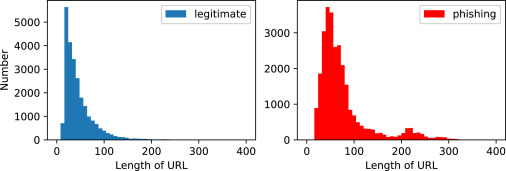
\includegraphics[width=0.9\textwidth]{url_length_50k.jpg}
	\caption{URL length distribution over a dataset of 50,000 records \citep{Li_Yukun}}
	\label{fig:URL_LENGTH_DISTRIBUTION}
\end{figure}

The second feature selected is the protocol used. There is a case to be made against utilising encryption usage due to its adoption growth shown by the \cite{APWG_Q42019}. However, although TLS adoption is growing, serving a website through HTTPS requires technical knowledge and a certain amount of effort. Besides this, the low average lifespan of a phishing webpage could help the average attacker decide against using it. Based on these factors, it is safe to assume that the number of phishing websites using TLS will not exceed 85\%. As of now, the protocol analysis on the dataset shows that the lack of TLS usage and maliciousness are highly correlated (Figure \ref{fig:FEATURE_CORRELATION}).

The third feature selected is the number of numerical characters in both the domain and subdomain. The choice comes from the fact that it is highly uncommon for benign domains and especially subdomains to contain any digits.

The fourth feature is the number of "@" and "\textasciitilde" characters. The reasoning behind this is that, like numerical characters, it is uncommon for an URL to contain these characters. The tilde is an outdated practice of accessing a user's folder on a Linux system by appending their name after the "\textasciitilde" character. The "@" is especially dangerous as it

\begin{singlespace}
	\begin{center}
		\begin{tabular}{  m{8em}  m{6em}  m{6em}  } \toprule

			                                             & \textbf{Benign} & \textbf{Phishing} \\ \midrule

			\multicolumn{1}{r}{\textbf{Average}}         & 57.81           & 77.54             \\

			\multicolumn{1}{r}{\textbf{Median}}          & 52              & 58                \\

			\multicolumn{1}{r}{\textbf{90th percentile}} & 90              & 143               \\

			\multicolumn{1}{r}{\textbf{95th percentile}} & 107             & 218               \\

			\multicolumn{1}{r}{\textbf{99th percentile}} & 141             & 321               \\ \bottomrule
		\end{tabular}
		\captionsetup{type=table}\caption{Statistical analysis of URL length over the training dataset}
		\label{tab:URL_SIZE_ANALISYS}
	\end{center}
\end{singlespace}

{\parindent0pt produces unexpected behaviour in the browser. It could either redirect to an email address using the default mail client or get the browser to ignore every character on its right side.}

The analysis of the dataset (Figure \ref{fig:FEATURE_CORRELATION}) shows that although they do not occur as often, these characters are still indicative of malicious activity and can improve decision-making.

The fifth feature is the presence of an additional network location in the URL. Given the popularity of hosting or storage services today and the existence of many open redirect vulnerabilities, some phishing URLs hide their real domain behind the trusted domain of another company. This feature flags up the presence of such practice by checking if the number of periods in the path of the URL exceeds one.

The sixth feature is chosen to be the number of hyphens. If there is no domain present in the path portion of the URL, the hyphen count is determined based on the network location only, otherwise for the whole URL. This method covers cases such as "target-brand.example.com" and "storage.service.com/website/target-brand.example.com/".

The seventh feature selected is the number of subdomains components. Most of the benign URLs either use "www" as subdomain or another arbitrary string of characters. However, the thing they have in common is that they mostly use only one subdomain component. In contrast, phishing URLs may use a multi-component subdomain to create the illusion of the target brand. Based on this reasoning, this feature will flag any URL whose subdomain components count exceeds two.

The eighth, ninth and tenth features flag the presence of sensitive vocabulary in the URL. \cite{Sujata_Garera} uncovered the correlation between a set of "sensitive" words and malicious intent in the study of phishing URL obfuscation techniques. The research was done in 2007; therefore, for maximising the efficiency of the word set, it needs to be extracted from an updated phishing URL list.
The word frequency count is performed on a compilation of multiple Phishtank lists of valid phishes. These are split in the format of "subdomain.domain/path?query". These sections are further probabilistically split using natural language processing (NLP) based on English Wikipedia unigram frequencies. Finally, the words that resulted from this process are sorted based on popularity.

Visual exploration of the sensitive vocabulary of the query segment shows that it overlaps with the one used in benign URLs, thus being prone to causing numerous false positives. Because of this, the final lists of sensitive words used are for the subdomain, domain and path section.

\begin{singlespace}
	\begin{center}
		\begin{tabular}{  m{13em}  m{13em}  } \toprule

			\textbf{Method}        & \textbf{Example result} \\ \midrule

			\textbf{Original}      & example.com             \\

			\textbf{Addition}      & examplea.com            \\

			\textbf{Bitsquatting}  & azample.com             \\

			\textbf{Homoglyph}     & ēxãmple.com             \\

			\textbf{Hyphenation}   & exampl-e.com            \\

			\textbf{Insertion}     & examplme.com            \\

			\textbf{Omission}      & exaple.com              \\

			\textbf{Repetition}    & exxample.com            \\

			\textbf{Replacement}   & esample.com             \\

			\textbf{Subdomain}     & ex.ample.com            \\

			\textbf{Transposition} & exapmle.com             \\

			\textbf{Vowel-swap}    & exomple.com             \\

			\textbf{TLD inclusion} & examplecom.com          \\ \bottomrule
		\end{tabular}
		\captionsetup{type=table}\caption{Domain variation techniques}
		\label{tab:VARIATIONS}
	\end{center}
\end{singlespace}

To further enhance the potential of this feature, the path and query sections of the URLs are searched for popular domains. Because it is a common practice in phishing URLs to use the target domain or brand in the path under the form of "www.example.com/ brand/signin.html", if there is no sensitive word found in the path, the first 2500 domains are searched throughout the path and query portions.

The last two features are based on the similarity index between the URL's domain and subdomain, and the top N benign domains. This feature directly targets the practice of brand obfuscation through mutations creating the surface illusion of accessing a trusted domain.
Phishing URLs use an array of techniques to create this illusion. A comprehensive list of these modifications is presented in Table \ref{tab:VARIATIONS}. All these variations aim to deceive the viewer if they do not exercise a closer inspection.

To capture such patterns, feature ten measures the Levenshtein distance between the target URL and the top 25,000 benign domains. The Levenshtein distance quantifies the difference between two strings by calculating the number of operations (deletion, insertion and substitution) needed to be performed on one of the strings for them to become identical. Naturally, a difference of zero means the strings are identical.

\begin{figure}[!t]
	\centering
	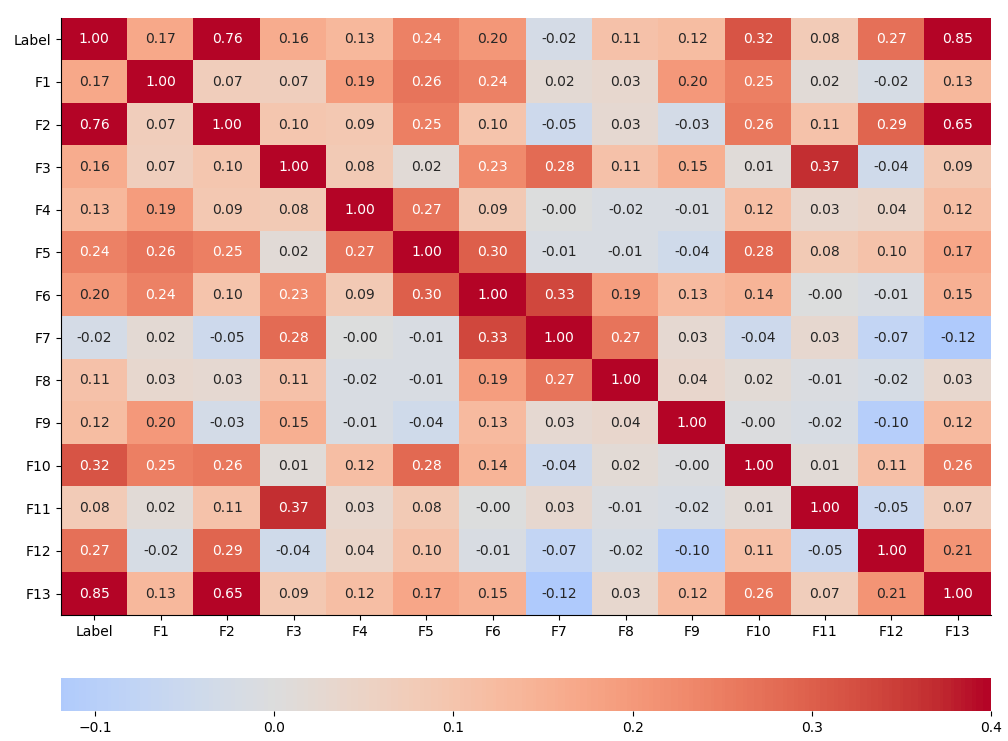
\includegraphics[width=1\textwidth]{feature_correlation.png}
	\caption{Correlation between labels and features}
	\label{fig:FEATURE_CORRELATION}
\end{figure}

\begin{singlespace}
	\begin{table}[b]
		\begin{center}
			\begin{tabular}{  m{13em}  m{10em}  } \toprule

				                                                    & \textbf{F1-score} \\ \midrule

				\multicolumn{1}{r}{\textbf{Naive Bayes}}            & 98.37\%           \\

				\multicolumn{1}{r}{\textbf{Decision Tree}}          & 98.74\%           \\

				\multicolumn{1}{r}{\textbf{Random Forest}}          & 98.86\%           \\

				\multicolumn{1}{r}{\textbf{Support Vector Machine}} & 98.76\%           \\

				\multicolumn{1}{r}{\textbf{Multi-layer Perceptron}} & 97.21\%           \\ \bottomrule
			\end{tabular}
			\caption{F-measure results of models training}
			\label{tab:FIRST_TRAINED_MODELS}
		\end{center}
	\end{table}
\end{singlespace}

The decision of using the Levenshtein distance is based on \cite{Mouad_Zouina}'s work, which showed that Levenshtein distance is the closest to the performance of Hamming distance in improving model predictions. Hamming distance does not fit the context of the artefact because it is designed to calculate distances between two strings of equal length. Also, Levenshtein distance covers the operations needed to perform all the mutations described in Table \ref{tab:VARIATIONS}. Finally, in case the Levenshtein distance is lower than six and different than zero, then the URL is flagged as suspicious.

The next feature applies the same process but on the extracted subdomain components. In this case, a distance lower than three will flag up the URL as suspicious. This is because subdomains closer to popular domain names are more suspicious than different variations of a domain. Moreover, zero distances are not ignored as these represent the presence of a benign domain in the subdomain components of the studied URL.

Looking at the correlations between the label (benign or malicious) and the feature set presented in this section (Figure \ref{fig:FEATURE_CORRELATION}), we can see how popular these practices are.

\begin{singlespace}
	\begin{table}[t]
		\begin{center}
			\begin{tabular}{  m{13em}  m{5em}  m{5em}  m{5em}  m{5em}  } \toprule

				                                & \textbf{Precision} & \textbf{Sensitivity} & \textbf{F1-score} & \textbf{Accuracy} \\ \midrule

				\textbf{Naive Bayes}            & 100\%              & 83.33\%              & 90.91\%           & 83.33\%           \\

				\textbf{Decision Tree}          & 100\%              & 81.15\%              & 89.59\%           & 81.15\%           \\

				\textbf{Random Forest}          & 100\%              & 82.11\%              & 90.17\%           & 82.11\%           \\

				\textbf{Support Vector Machine} & 100\%              & 78.91\%              & 88.21\%           & 78.91\%           \\

				\textbf{Multi-layer Perceptron} & 100\%              & 82.69\%              & 90.52\%           & 82.69\%           \\ \bottomrule
			\end{tabular}
			\captionsetup{type=table}\caption{Initial models tested with Phishtank data (1st of April)}
			\label{tab:PERFORMANCE_ASSESSMENT}
		\end{center}
	\end{table}
\end{singlespace}

\section{Initial performance assessment}
This section follows the process of model training and initial performance assessment. The results of training the first set of models show the remarkable synergy between the features. Table \ref{tab:FIRST_TRAINED_MODELS} presents the F1 scores of the algorithms. The F1-score is chosen as the representative metric because it is fit for generalising performance.

\begin{figure}[!b]
	\centering
	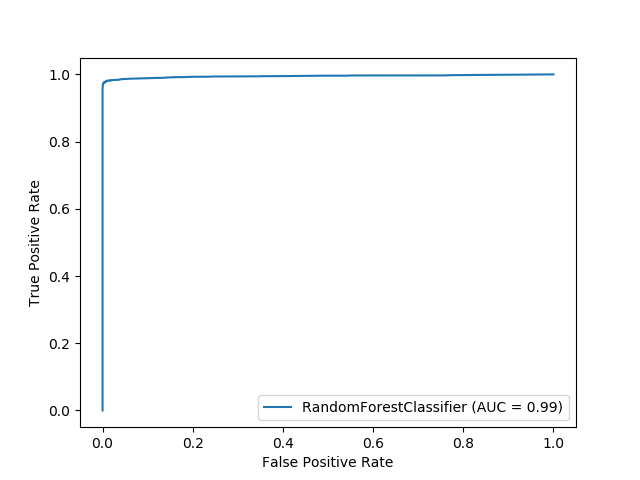
\includegraphics[width=0.49\textwidth]{rf_example_roc.png}
	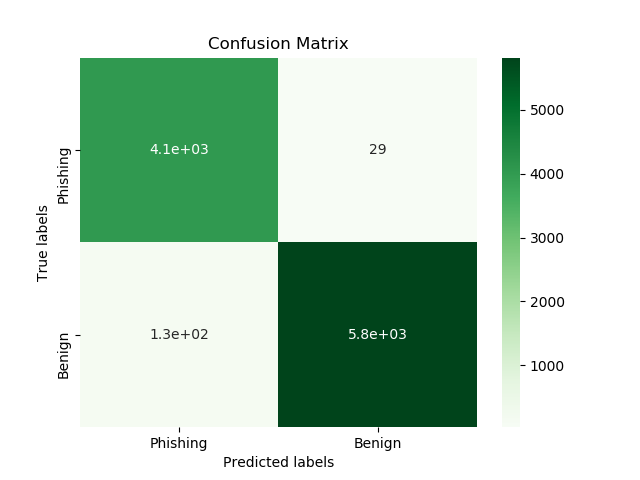
\includegraphics[width=0.49\textwidth]{rf_example_cm.png}
	\caption{ROC and confusion matrix of the random forest model}
	\label{fig:ROC_CM_EXAMPLE}
\end{figure}

Figure \ref{fig:ROC_CM_EXAMPLE} presents both the ROC and confusion matrix for the Random Forest model. The 0.99 value of the area under the curve (AUC) points out that the model can easily distinguish between the two classes of URLs. The confusion matrix reveals that it is uncommon for the model to mislabel URLs. The example shows that the random forest mislabeled 109 URLs out of 10,000.

Next, the models deliver predictions on the remainder benign and phishing of the 450,000 URLs dataset to test its performance in a realistic scenario. The results collected from the predictions over 305,737 benign URLs and 74,436 phishing URLs are presented in Table \ref{tab:PERFORMANCE_ASSESSMENT}.



The next dataset used to evaluate model performance is composed of online and valid phishes from 1st of April. This way, the models are tested with the same parameters Google safe browsing was.


\section{Performance improvement}
Given the results of the models presented in the previous section, the performance improvement shown in this section is not expected to be substantial.
The first step in improving the performance is removing features with a correlation to the label close to zero. The correlation heatmap presented in Figure \ref{fig:FEATURE_CORRELATION} shows feature number seven as having the lowest correlation to the label. Removing the long subdomain feature reduces confusion in model training and offers a slight improvement in delivering more accurate predictions. Figure \ref{fig:IMPROVED_FEATURE_CORRELATION} illustrates the correlation heatmap after removal.

\begin{figure}[!b]
	\centering
	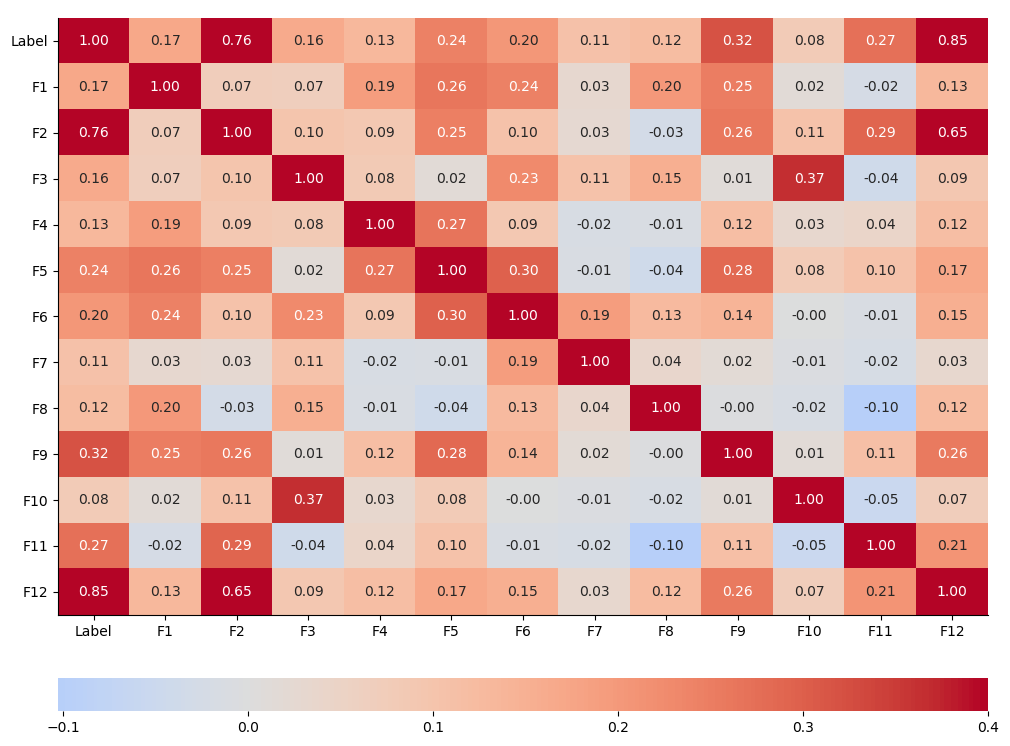
\includegraphics[width=1\textwidth]{improved_feature_correlation.png}
	\caption{Improved feature correlation heatmap}
	\label{fig:IMPROVED_FEATURE_CORRELATION}
\end{figure}

The second step is hyperparameter tuning. The process of hyperparameter tuning or optimisation consists of training the subject model with different values for its parameters. Trying different permutations of values for these parameters influences prediction quality, thus finding the right combination improves overall performance.

Hyperparameter tuning is computationally expensive. Because of this, the algorithms selected for optimisations are the ones that already deliver superior and consistent results. These are the random forest, the support vector machine and the multi-layer perceptron classifiers.

\begin{singlespace}
	\begin{table}
		\begin{center}
			\begin{tabular}{  m{13em}  m{5em}  m{10em}  m{2.3em} }\toprule

				                                & \textbf{F1-score} & \textbf{F1-score (optimised)} & \textbf{Delta} \\ \midrule

				\textbf{Random Forest}          & 98.86             & 98.92                         & 0.08           \\

				\textbf{Support Vector Machine} & 98.76             & 98.87                         & 0.11           \\

				\textbf{Multi-layer Perceptron} & 97.21             & 98.76                         & 1.25           \\ \bottomrule
			\end{tabular}
			\captionsetup{type=table}\caption{Comparison of optimised models}
			\label{tab:OPTIMISED_MODELS}
		\end{center}
	\end{table}
\end{singlespace}

In the tuning of the random forest classifier, the number of n\_estimators is increased to raise the number of decision trees. By doing so, the model can deliver better predictions at the expense of both training and prediction time. Because of this, the number of n\_estimators is set to either 150, 295 or 350. Next, the max\_depth of each decision tree is set to be either 15,18 or 21. The last optimisation is done on the max\_features parameter. This sets the number of maximum features provided to each tree and will be tested with the values of auto and sqrt.

The calibration of the SVM classifier is done by searching for the best performing C parameter. The C parameter influences the misclassification threshold of the model. With a greater C value, the classifier will choose a smaller-margin hyperplane, rendering the model less prone to delivering wrong predictions. However, a bigger C value will increase the chance of overfitting. Finally, the values of the C fed into the GridSearchCV are 10,100 and 1000.

Given the opaque nature of the training process of neural networks, the calibration of the multi-layer perceptron matches hit-or-miss experimentation. Because of this, different models have been trained using most of the calibration parameters that the MLP classifier takes as input (Appendix \ref{appendix:model_configurations}).


\begin{figure}[!b]
	\centering
	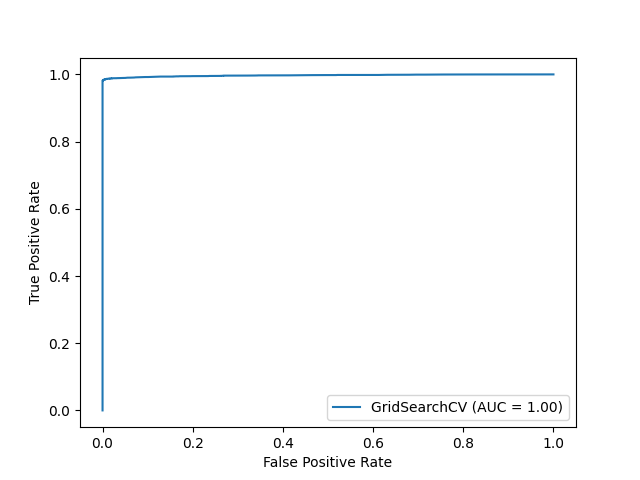
\includegraphics[width=0.49\textwidth]{random_forest_calibrated_roc.png}
	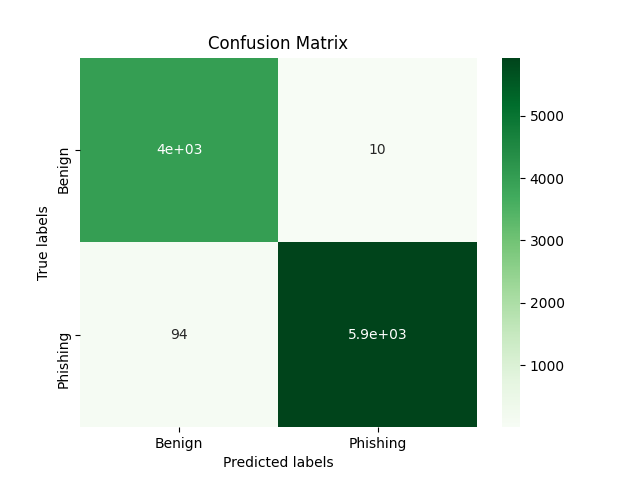
\includegraphics[width=0.49\textwidth]{random_forest_calibrated_cm.png}
	\caption{ROC and confusion matrix of the random forest model}
	\label{fig:OPTIMISED_RF}
\end{figure}

As expected, the results of the optimisation did not deliver a substantial improvement. Table \ref{tab:OPTIMISED_MODELS} shows that the best model to include in our final classifier is random forest. However, before venturing to do so, additional testing needs to be performed to ensure the model is not overfitted. For this, the remainder of the initial dataset is used. Table \ref{tab:FINAL_MODEL} shows that not only the model is not overfitted, but the accuracy is higher by 0.35\% than the one reported during training.

\begin{singlespace}
	\begin{table}
		\begin{center}
			\begin{tabular}{ m{9em} m{5em} } \toprule
				\textbf{Metric}      & \textbf{Value} \\ \midrule

				\textbf{Precision}   & 97.40\%        \\

				\textbf{Sensitivity} & 99.06\%        \\

				\textbf{F-measure}   & 98.22\%        \\

				\textbf{Accuracy}    & 99.29\%        \\ \bottomrule
			\end{tabular}
			\captionsetup{type=table}\caption{ Optimised random forest results on the 380,000 mixed records dataset}
			\label{tab:FINAL_MODEL}
		\end{center}
	\end{table}
\end{singlespace}

An important factor in model selection and calibration is the number of false positives produces. Higher delivery of false positives leads to less trust in alerts on the user's side. Because of this, the final model needs to prioritise precision over recall and false negatives over false positives.

The confusion matrix (Figure \ref{fig:OPTIMISED_RF}) proves that the final random forest model fulfils this aim by having a 0.10\% rate of false positives.

\section{Chapter overview}
The design and implementation chapter described the modules of the classifier and justified the decision. It also explored the features chosen in great detail and presented an initial performance assessment. Based on the results of this assessment, the features have been tweaked to improve the machine learning model. Finally, the chapter closes with a compelling set of metrics reported by the improved model.